\documentclass{article}

\usepackage{tikz}
\usetikzlibrary{calc, positioning, fit, backgrounds, spy, decorations.pathreplacing, chains}

\usepackage{pgfplots}
\pgfplotsset{compat=1.16}

\begin{document}

% Define pastel colors
\definecolor{pastelblue}{RGB}{179,205,227}
\definecolor{pastelorange}{RGB}{251,180,174}
\definecolor{pastelgreen}{RGB}{170, 210, 170}

\def\width{1.2}
\def\height{0.5}
\def\sgma{1.0}

\tikzset{
    rect/.style={
        % draw,
        minimum width=\width cm,
        minimum height=\height cm,
        thick,
        align=center
    }
}

% draw vehicles on one route
\def\routespace{1.2} % space between route rows
\newcommand{\route}[5]{%
  % #1 = route id, #2 = number of vehicles, #3 = start x, #4 = color, #5 = average gap
  \pgfmathsetmacro{\xl}{#3}
  \foreach \k in {1,...,#2} {
    \pgfmathsetmacro{\y}{-\routespace * (#1 - 1)}
    \node[rect, draw, thin, fill=#4] (#1-\k) at (\xl + \width / 2,\y) {};% {(#1,\k)};
    \pgfmathparse{\xl + \width + rnd*#5}
    \global\let\xl\pgfmathresult
  }
}

\centering

\section*{Partial schedule and horizon}


\begin{tikzpicture}
\pgfmathsetseed{1}
\pgfmathsetmacro{\x}{-6.5}
\def\y{0}
\foreach \i/\gap/\color in {
  1/0/pastelorange,
  2/\sgma/pastelorange,
  3/0.4/pastelblue,
  4/0/pastelblue%
} {
  \node[rect, thin, draw=black!50, fill=\color!50] (\i) at (\x, \y) {};
  \pgfmathparse{\x + \width + \gap}
  \global\let\x\pgfmathresult
}
% draw switchover time
\draw[->, >=stealth, draw=black!50, text=black!50] (2) -- node[midway, above] {$\sigma$} (3);

% % indicate the partial schedule that is "done"
% \draw [decorate,decoration={brace,amplitude=5pt}]
%   ([yshift=4pt] 1.north west) -- ([yshift=4pt] 4.north east)
%   node[midway,yshift=12pt]{partial schedule};

% % indicate "horizon"
% \draw [decorate,decoration={brace,amplitude=5pt}]
%   ([xshift=2pt, yshift=4pt] 4.north east) -- ($([yshift=4pt] 4.north east) + (6, 0)$)
%   node[midway,yshift=12pt]{horizon};

% set x to end of last scheduled vehicle
\pgfmathsetmacro{\xend}{\x - \width / 2}

% draw current time line
\draw[dashed] (\xend, -\height) -- (\xend, -3.0);

% draw upcoming vehicles of same route
\route{1}{3}{\xend + 0.3}{pastelblue}{0.8}

% draw upcoming vehicles of other routes
\pgfmathsetmacro{\x}{\xend + \sgma}
\route{2}{2}{\x + 0.5}{pastelorange}{5.0}
\route{3}{3}{\x}{pastelgreen}{0.8}

% draw sigma arrows for other routes
\draw[->,>=stealth, ] (\xend, -\routespace) -- node[midway, above] {$\sigma$} ($(\xend, -\routespace) + (\sgma, 0)$) ;
\draw[->,>=stealth, ] (\xend, -2*\routespace) -- node[midway, above] {$\sigma$} ($(\xend, -2*\routespace) + (\sgma, 0)$) ;

% draw grey route boxes
\begin{pgfonlayer}{background}
  % \node[fill=gray!15, rounded corners, fit=(1)(4), inner sep=0.2cm] {};
  % \node[fill=gray!15, rounded corners, fit=(2-1)(2-5), inner sep=0.2cm] {};
  % \node[fill=gray!15, rounded corners, fit=(3-1)(3-5), inner sep=0.2cm] {};
\end{pgfonlayer}

\end{tikzpicture}


\section*{Complete schedule example}

% draw vehicles on one route
\def\routespace{1.2} % space between route rows
\newcommand{\schedule}[3]{%
  % #1 = alternations, #2 = max number of vehicles, #3 = average gap

  % specify colors to alternate between
  \def\colors{pastelorange,pastelblue}
  \def\ncolors{2}

  % keep track of the x position of vehicles
  \pgfmathsetmacro{\x}{0}

  % for specified number of "alternations"
  \foreach \r in {1,...,#1} {
    % alternate between colors
    \pgfmathtruncatemacro{\idx}{mod(\r-1, \ncolors) + 1}

    % loop trough colors and count (like enumerate(colors) in python)...
    \foreach \col [count=\j] in \colors {
      \ifnum \j=\idx
        % ...do this because we cannot simply do array indexing

        % sample random number of vehicles in this "burst"
        \pgfmathrandominteger{\n}{1}{#2}
        % draw these vehicles
        \foreach \k in {1,...,\n} {
            % random gap, but not too small
            \pgfmathsetmacro{\nogap}{rnd}
            \pgfmathparse{\nogap < 0.2}
            \ifnum \pgfmathresult=1
              % set 0 if too smal
              \pgfmathsetmacro{\gap}{0}
            \else
              \pgfmathsetmacro{\gap}{0.2 + rnd*#3}
            \fi

            % gap is mininum of sigma when k=1
            \ifnum \k=1
              \pgfmathparse{\gap < \sgma}
              \ifnum \pgfmathresult=1
                \pgfmathsetmacro{\gap}{\sgma}
              \fi
            \fi

            \pgfmathparse{\x + \width + \gap}
            \global\let\x\pgfmathresult

            % draw switchover time
            \ifnum \r=#1\else % (but not for the last vehicle of last route)
            \ifnum \k=\n % for last vehicle
            \draw[->, >=stealth, draw] (\x + \width, 0) -- node[midway, above] {$\sigma$} (\x + \width + \sgma, 0);
            \fi
            \fi

            \node[rect, draw, thin, fill=\col] (\r-\k) at (\x + \width / 2, 0) {};% {(#1,\k)};
        }
      \fi
    }
  }
}

\begin{figure}[h]
\centering
\begin{tikzpicture}
  \pgfmathsetseed{9023}
  \def\width{0.8}
  \def\height{0.3}
  \def\sgma{1.0}
  \schedule{4}{4}{0.3}
\end{tikzpicture}
\end{figure}



\section*{Recurrent neural network}

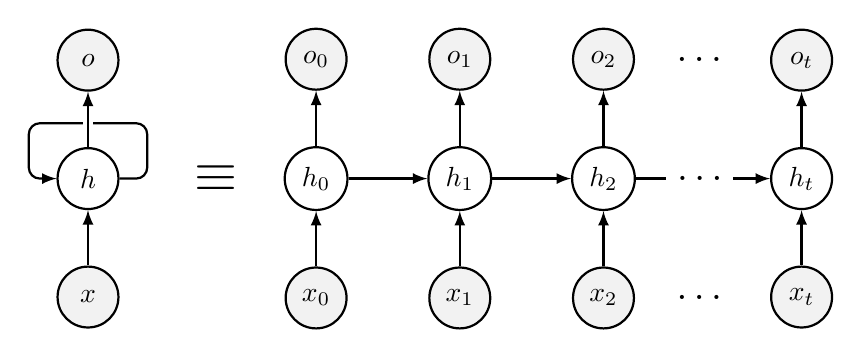
\begin{tikzpicture}[item/.style={circle,draw,thick,align=center, minimum size=2.2em},
itemc/.style={item,on chain,join}]
 \begin{scope}[start chain=going right,nodes=itemc,every
 join/.style={-latex,thick},local bounding box=chain]
 \path node (A0) {$h_0$} node (A1) {$h_1$} node (A2) {$h_2$} ;
 \end{scope}
 \node[circle, draw,thick, align=center, minimum size=2.2em, xshift=2em, on chain] (At) {$h_t$};

 \draw[thick] (A2) -- ($(A2) + (0.8,0)$);
 % \draw[thick,dashed] ($(A2) + (0.7,0)$) -- ($(A2) + (1.6,0)$);
 \draw[thick,-latex] ($(A2) + (1.65,0)$) -- (At);

 \node[left=1em of chain,scale=2] (eq) {$\equiv$};

 \node[left=2em of eq,item] (AL) {$h$};
 \path (AL.west) ++ (-1em,2em) coordinate (aux);
 \draw[thick,-latex,rounded corners] (AL.east) -| ++ (1em,2em) -- (aux)
 |- (AL.west);

 \foreach \X in {0,1,2,t} {

 \draw[thick,-latex] (A\X.north) -- ++ (0,2em)
 node[above,item,fill=gray!10] (o\X) {$o_\X$};

 \draw[thick,latex-] (A\X.south) -- ++ (0,-2em)
 node[below,item,fill=gray!10] (x\X) {$x_\X$};

 }

 \path (x2) -- (xt) node[midway,scale=1.4] {\dots};
 \path (o2) -- (ot) node[midway,scale=1.4] {\dots};
 \path (A2) -- (At) node[midway,scale=1.4] {\dots};

 \draw[white,line width=0.8ex] (AL.north) -- ++ (0,1.9em);

 \draw[thick,-latex] (AL.north) -- ++ (0,2em)
 node[above,item,fill=gray!10] {$o$};

 \draw[thick,latex-] (AL.south) -- ++ (0,-2em)
 node[below,item,fill=gray!10] {$x$};

\end{tikzpicture}


\clearpage
\begin{tikzpicture}[
    spy using outlines={rectangle, magnification=1.4,
      spy connection path={
        \draw[thin] (tikzspyonnode.south east) -- (tikzspyinnode.north east);
        \draw[thin] (tikzspyonnode.south west) -- (tikzspyinnode.north west);
    }}
]

\tikzset{
    rect/.style={rounded corners=6pt, minimum width=2.5cm, minimum height=1.2cm, align=center}
}

\node[rect, fill=pastelblue] (r1) {Step 1};
\node[rect, fill=pastelgreen, right=1.2cm of r1] (r2) {Step 2};
\node[rect, fill=pastelorange, right=1.2cm of r2] (r3) {Step 3};

\node[draw, dashed, rounded corners, fit=(r2)(r3), inner sep=0.2cm] (zoombox) {};

\spy [blue, width=10cm, height=3cm] on (zoombox) in node [below=2cm of r3,xshift=-3cm] ;

\end{tikzpicture}

\end{document}
